\documentclass[a4paper,12pt]{article}
\usepackage[a4paper, margin=2.5cm]{geometry}
\usepackage[pdftex]{graphicx}
\usepackage{tikz}
\usepackage{pgfplots}
\usepackage{enumitem}
\usepackage{float}
\usepackage[document]{ragged2e}
\usepackage[utf8]{inputenc}
\usepackage[T1]{fontenc}
\usepackage[spanish,es-tabla]{babel}
\renewcommand{\shorthandsspanish}{}
\usepackage{xurl}
\usepackage{lipsum}
\usepackage{mwe}
\usepackage{multirow}
\usepackage{multicol}
\usepackage{siunitx}
\usepackage{listings}
\usepackage{circuitikz}
\usepackage{tabularray}
\usepackage{amsmath}
\usepackage{gensymb}


\usetikzlibrary{arrows.meta,bending}
\graphicspath{ {/home/saikkopat/Documents/school/CE/'Tarea CA'/figures/} }

\title{Tarea: Introducción a la corriente alterna}
\author{González Cárdenas Ángel Aquilez \and Sánchez González Daniel Iván}

\begin{document}

\begin{titlepage}
	\begin{tikzpicture}[overlay, remember picture]
		\path (current page.north east) ++(-0.3,-1.5) node[below left] {
\includegraphics[width=0.35\textwidth]{/home/saikkopat/Documents/LOGOS IPN/EscudoESCOM}};
	\end{tikzpicture}
	\begin{tikzpicture}[overlay, remember picture]
		\path (current page.north west) ++(1.5,-1) node[below right] {
\includegraphics[width=0.2\textwidth]{/home/saikkopat/Documents/LOGOS IPN/logo}};
	\end{tikzpicture}
	\begin{center}
		\vspace{-1.5cm}
		{\LARGE Instituto Politécnico Nacional\par}
		\vspace{.5cm}
		{\LARGE Escuela Superior de Cómputo\par}
		\vspace{2cm}
		{\large Unidad de aprendizaje:}\\{\Large Circuitos Eléctricos\par}
		\vspace{2cm}
		{\scshape\Huge Tarea:\par}
		{\itshape\Large Números complejos, capacitor e inductor\par}
		\vfill
		\vspace{.7cm}
		{\Large Grupo: 3CV2\par}
		\vspace{.7cm}
		{\Large Integrantes:\\González Cárdenas Ángel Aquilez\\Sánchez González Daniel Iván\par}
		\vspace{1cm}
		{\Large Profesor: Vázquez Ortiz Mijail\par}
		\vspace{1cm}
		{\large Fecha de entrega: 6 de junio de 2023\par}
		\vfill
	\end{center}
\end{titlepage} 

\newpage

\usepgfplotslibrary{units}


\section*{Números complejos}

\begin{enumerate}
	\item ¿Qué son los números complejos? \\ Según Stewart, Redlin y Watson:
	\begin{quotation}
		Un número complejo es una expresión de la forma
		\[a + bi\]
		donde $a$ y $b$ son números reales y $i^2 = -1$. La parte \emph{real} de este número complejo es $a$ y la parte \emph{imaginaria} es $b$. Dos números complejos son iguales si y sólo si sus partes reales son iguales y sus partes imaginarias son iguales.
	\end{quotation}
	Cómo $i^2 = -1$, se tiene que $i = \sqrt{-1}$, siendo esta la base para el sistema numérico expandido llamado \emph{sistema de números complejos}.
	
	\item Representación polar de los números complejos.\\ Un número complejo $z = a + bi$ tiene la \emph{forma polar} (o forma trigonométrica) si se representa como:
	\[z = r(\cos \theta + i \sen \theta)\]
	donde $r = |z| = \sqrt{a^2 + b^2}$ y $\tan \theta = \dfrac{b}{a}$. El número $r$ es el \emph{módulo} de $z$ y $\theta$ es un \emph{argumento} de $z$. \\
	También nos es posible representar un número complejo de la forma \[z = r \angle \theta\] donde $\theta = \arctan \dfrac{b}{a}$, y si un número complejo aparece representado en cualquier otro cuadrante que no fuese el primero, se deberá convertir de forma apropiada.\\
	\vspace{0.5cm}
	Ejemplos: (a) $1 + i$, (b) $-1 + \sqrt{3} i$, (c) $-4\sqrt{3} -4i$ \\


	\begin{figure}[!h]
	\centering
		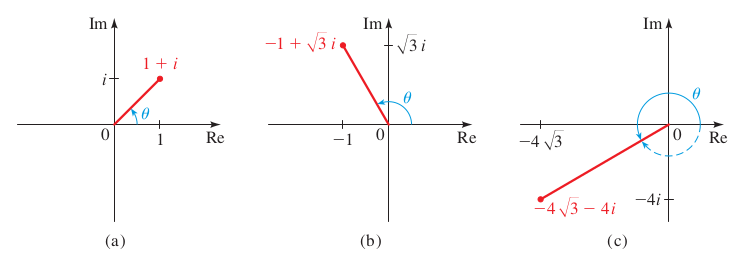
\includegraphics[width=.8\textwidth]{fig1}
		\label{fig1}
		\caption{Ejemplos de números complejos en forma polar}
	\end{figure}

	\item Representación rectangular de los números complejos \\ La representación \emph{rectangular} de un número complejo está dada por \[z = a + bi\]
	Ejemplos: (a) $3 + 4i$ (b) $\dfrac{1}{2} - \dfrac{2}{3} i$ (c) $6i$

	\item Conversiones entre representaciones polar y rectangular \\ Para convertir un número complejo de su representación rectangular a polar partimos de lo indicado en (2) y de la Figura 1: \\
	(a) Haciendo a $1 + i$ a su representación polar, tenemos que $r = \sqrt{1 + 1} = \sqrt{2}$ y $\arctan \dfrac{1}{1} = \arctan 1 = 45\degree$, por lo tanto \[1 + i = \sqrt{2} \angle 45\degree\] 
	(b) Para $-1 + \sqrt{3}i$, tenemos que $r = \sqrt{1 + 3} = 2$ y $\arctan \dfrac{\sqrt{3}}{-1} = \arctan -\sqrt{3} = -60\degree$, pero para conseguir $\theta$ hacemos \[\theta = 180\degree - 60\degree = 120\degree\] por lo tanto \[-1 + \sqrt{3}i = 2 \angle 120\degree\] 
	(c) Para $-4\sqrt{3} - 4i$ a su representación polar, tenemos que $r = \sqrt{48 + 16} = 8$ y $\arctan \dfrac{-4}{-4\sqrt{3}} = \arctan \dfrac{1}{\sqrt{3}} = 30\degree$, luego $\theta = 180\degree + 30\degree = 210\degree$ Así \[-4\sqrt{3} - 4i = 8 \angle 210\degree\] 

	Luego, para convertir un número complejo de su representación polar a rectangular hacemos: 
	\[a = r \cos \theta\]
	\[b = r \sen \theta\]
	Para los ejemplos tenemos que \\
	(a)$\sqrt{2} \angle 45\degree$ a su representación rectangular, $a = \sqrt{2} \cos 45\degree = \sqrt{2} \dfrac{\sqrt{2}}{2} = 1$, y para $b = \sqrt{2} \sen 45\degree = \sqrt{2} \dfrac{\sqrt{2}}{2} = 1$. Por lo tanto \[\sqrt{2} \angle 45\degree = 1 + i\]
	(b) De $2 \angle 120\degree$ a su representación rectangular, $a = 2 \cos 120\degree = 2 \dfrac{-1}{2} = -1$, y para $b = \sqrt{2} \sen 120\degree = 2 \dfrac{\sqrt{3}}{2} = \sqrt{3}$. Así \[ 2 \angle 120\degree = -1 + \sqrt{3}i\]
	(b) Finalmente para $8 \angle 210\degree$ se tiene que $a = 8 \cos 210 = 8 \dfrac{-\sqrt{3}}{2} = -4\sqrt{3}$ y para $b = 8 \sen 210 = 8 \dfrac{-1}{2} = -4$. Así \[8 \angle 240\degree = -4\sqrt{3} -4i\]
	\vspace{0.5cm}

	\item Operaciones de suma, resta, división y multiplicación de números complejos \\ 
	
	\begin{enumerate}
		\item Suma: para sumar dos o más números complejos se suman las partes reales e imaginarias por separado.
		\[C_1 + C_2 = (a_1 + a_2) + i(b_1 + b_2)\]
		Ejemplos:\\
		\begin{enumerate}
			\item $C_1 = 5+10i$ y $C_2 = 2+6i$ \\
			Así \[C_1 + C_2 = (5+2) + i(10+6) = 7 + 16i\]
			\item $C_1 = 8+15i$ y $C_2 = -7+8i$ \\
			Así \[C_1 + C_2 = (8-7) + i(15+8) = 1 + 23i\]
			\item $C_1 = -27+3i$ y $C_2 = 30-15i$ \\
			Así \[C_1 + C_2 = (-27+30) + i(3-15) = 3 - 12i\]
		\end{enumerate}

	Es importante recordar que la adición o sustracción no pueden realizarse en forma polar a no ser que los números complejos tengan el mismo ángulo, o a menos que difieran sólo por múltiplos de 180°. \\

	Ejemplos:\\
		\begin{enumerate}
			\item $C_1 = 4 \angle 60\degree$ y $C_2 = 1 \angle 60\degree$ \\
			Así \[C_1 + C_2 = 4+1 \angle 60\degree = 5 \angle 60\degree \]
			\item $C_1 = 12 \angle 90\degree$ y $C_2 = 3 \angle 90\degree$ \\
			Así \[C_1 + C_2 = 12+3 \angle 90\degree = 15 \angle 60\degree \]
			\item $C_1 = -4 \angle 120\degree$ y $C_2 = -5 \angle 120\degree$ \\
			Así \[C_1 + C_2 = -4-5 \angle 120\degree = -9 \angle 120\degree \]
		\end{enumerate}



	\item Resta: para restar dos o más números complejos se restan las partes reales e imaginarias por separado.
		\[C_1 - C_2 = (a_1 - a_2) + i(b_1 - b_2)\]
		Ejemplos:\\
		\begin{enumerate}
			\item $C_1 = 10+3i$ y $C_2 = 6+4i$ \\
			Así \[C_1 - C_2 = (10-6) + i(3-4) = 4 - i\]
			\item $C_1 = -6+15i$ y $C_2 = 6+20i$ \\
			Así \[C_1 - C_2 = (-6 -6) + i(15-20) = -12 -5i\]
			\item $C_1 = -7-5i$ y $C_2 = -8+i$ \\
			Así \[C_1 - C_2 = (-7+8) + i(-5-1) = 1 - 6i\]
		\end{enumerate}
	Y para la representación polar tenemos:\\
		\begin{enumerate}
			\item $C_1 = 4 \angle 60\degree$ y $C_2 = 1 \angle 240\degree$ \\
			Así \[C_1 - C_2 = 4-1 \angle 60\degree = 3 \angle 60\degree \]
			\item $C_1 = 3 \angle 90\degree$ y $C_2 = 12 \angle 270\degree$ \\
			Así \[C_1 - C_2 = 3-12 \angle 90\degree = -9 \angle 270\degree \]
			\item $C_1 = -4 \angle 120\degree$ y $C_2 = -5 \angle -60\degree$ \\
			Así \[C_1 - C_2 = -4+5 \angle 120\degree = 1 \angle 120\degree \]
		\end{enumerate}

	\item Multiplicación: Para multiplicar dos números complejos en su representación rectangular se multiplica las partes real e imaginaria una a la vez por las partes real e imaginaria del otro: 
	\[C_1 \times C_2 = (a_1 a_2 - b_1 b_2) + i(b_1 a_2 + a_1 b_2)\]
	Ejemplos:\\
		\begin{enumerate}
			\item $C_1 = 4+5i$ y $C_2 = 10+15i$ \\
			Así \[C_1 \times C_2 = [4(10) - 5(15)] + i[5(10) + 4(15)] = -35 + 110i\]
			\item $C_1 = -2-3i$ y $C_2 = 4-6i$ \\
			Así \[C_1 \times C_2 = [-2(4) - 3(6)] + i[-3(4) + 2(6)] = -26 + 0i\]
			\item $C_1 = 5+5i$ y $C_2 = -4-4i$ \\
			Así \[C_1 \times C_2 = [5(-4) - 5(-4)] + i[-4(5) + 5(-4)] = -40i\]
		\end{enumerate}
	En la representación polar, las magnitudes se multiplican y los ángulos se suman algebraicamente.
	\[C_1 \times C_2 = z_1 \times z_2 \angle {\theta}_1 + {\theta}_2\] \\
	Ejemplos:\\
		\begin{enumerate}
			\item $C_1 = 5 \angle 20\degree$ y $C_2 = 10 \angle 30\degree$ \\
			Así \[C_1 \times C_2 = 5(10) \angle 20\degree + 30\degree = 50 \angle 50\degree\]
			\item $C_1 = 2 \angle -40\degree$ y $C_2 = 7 Q\angle 120\degree$ \\
			Así \[C_1 \times C_2 = 2(7) \angle -40\degree + 120\degree = 14 \angle 80\degree\]
			\item $C_1 = -10 \angle 90\degree$ y $C_2 = 6 \angle 180\degree$ \\
			Así \[C_1 \times C_2 = -10(6) \angle 90\degree + 180\degree = -60 \angle 270\degree\]
		\end{enumerate}
	Para multiplicar un número complejo en forma rectangular por un número real se requiere que tanto la parte real como la imaginaria se multipliquen por el número real: \\
	\[3(4 + 5i) = 12 + 15i\]
	\[25 \angle 0\degree (0 + 3i) = 75i = 75 \angle 90\degree\]
	\[8 \angle 0\degree (2 + 4i) = 16 + 32i \approx 35.77 \angle 63.43\degree\]

	\item División: Para dividir dos números complejos en forma rectangular, multiplique el numerador y denominador por el conjugado del denominador y las partes reales e imaginarias se reúnen:

	\[\frac{C_1}{C_2} = \frac{a_1 a_2 + b_1 b_2}{a_2 ^2 + b_2 ^2} + i\frac{a_2 b_1 - a_1 b_2}{a_2 ^2 + b_2 ^2}\]
	Ejemplos:\\
		\begin{enumerate}
			\item $C_1 = 1+4i$ y $C_2 = 4+5i$ \\
			Así \[\frac{C_1}{C_2} = \frac{1(4) + 4(5)}{4^2 + 5^2} + i\frac{4(4) - 1(5)}{4^2 + 5^2} = \frac{24}{41} + \frac{11}{41}i\]
			\item $C_1 = -4-8i$ y $C_2 = 6-1i$ \\
			Así \[\frac{C_1}{C_2} = \frac{-4(6) + 8(1)}{6^2 - 1^2} + i\frac{6(-8) - 4(1)}{6^2 - 1^2} = \frac{-16}{37} + \frac{-52}{37}i\]
			\item $C_1 = 2+3i$ y $C_2 = 4+6i$ \\
			Así \[\frac{C_1}{C_2} = \frac{2(4) + 3(6)}{4^2 + 6^2} + i\frac{4(3) - 2(6)}{4^2 + 6^2} = \frac{26}{52} + 0i = \frac{1}{2}\]
		\end{enumerate}
	Para la representación polar, la división se realiza  dividiendo la magnitud del numerador entre la magnitud del denominador y restando el ángulo del denominador del ángulo del numerador:
	\[\frac{C_1}{C_1} = \frac{z_1}{z_2}\angle {\theta}_1 - {\theta}_2\] \\
	Ejemplos:\\
		\begin{enumerate}
			\item $C_1 = 15 \angle 10\degree$ y $C_2 = 2 \angle 7\degree$ \\
			Así \[\frac{C_1}{C_2} = \frac{15}{2} \angle 10\degree - 7\degree = 7.5 \angle 3\degree\]
			\item $C_1 = 8 \angle 120\degree$ y $C_2 = 16 \angle -150\degree$ \\
			Así \[\frac{C_1}{C_2} = \frac{8}{16} \angle 120\degree - (-150\degree) = 0.5 \angle 270\degree\]
			\item $C_1 = 50 \angle 30\degree$ y $C_2 = 2 \angle 20\degree$ \\
			Así \[\frac{C_1}{C_2} = \frac{50}{2} \angle 30\degree - 20\degree = 25 \angle 10\degree\]
		\end{enumerate}
	\end{enumerate}

\end{enumerate}

\section*{Capacitor}
\begin{enumerate}
\item Definición de \emph{condensador} o \emph{capacitor}: \\ Según Hayt \emph{et al}:\\
\begin{quotation}
	Es un dispositivo [eléctrico] que se compone de dos superficies conductoras sobre las que puede almacenarse una carga, y están separadas por una delgada capa aislante que tiene una resistencia muy grande.
\end{quotation}
	Además, según Boylestad \emph{et al}: 
	\begin{quotation}
		Un capacitor tiene una capacitancia de $\SI{1}{\farad}$ si se deposita $\SI{1}{\coulomb}$ de carga ($6.242 \times 10^18$ electrones) en las placas, por una diferencia de potencial de $\SI{1}{\volt}$ a través de sus placas.
	\end{quotation}

	\item ¿Qué es \emph{capacitancia}? \\ 
	Para Boylestad \emph{et al}:\\
	\begin{quotation}
		Es la medida de la capacidad de un capacitor de almacenar carga en sus placas... Cuanto más alta es la capacitancia de un capacitor, más grande es la cantidad de carga almacenada en las placas con el mismo voltaje aplicado.
	\end{quotation}

	\item Tipos de capacitores: \\
	Existen dos tipos de capacitores: \emph{fijos} y \emph{variables}. De forma similar a los resistores, se utilizan los siguientes símbolos para denotarlos:\\
	
	\begin{figure}[h!]
		\centering

		\begin{multicols}{2}
			\begin{circuitikz}[american, voltage dir=RP]
				\draw (0,0)
				to[C] ++(2,0);
			\end{circuitikz}
			\vspace{0.3cm}
		\\(A) fijo

		\columnbreak

			\begin{circuitikz}[american, voltage dir=RP]
				\draw (0,0)
				to[vC] ++(2,0);
			\end{circuitikz}
			\vspace{0.3cm}
		\\(B) variable
		\end{multicols}
		\caption{Símbolos del capacitor}
	\end{figure}

	\item Capacitores en serie y paralelo:\\
	Para determinar la capacitancia equivalente de $n$ capacitores en serie utilizamos:
	\[C_{eq} = \dfrac{1}{\dfrac{1}{C_1} + \dfrac{1}{C_2} + ... \dfrac{1}{C_n}}\]
	Y cuando tenemos solo dos elementos utilizamos:
	\[C_{eq} = \dfrac{C_1 C_2}{C_1 + C_2}\]
	Ejemplos: determine la capacitancia equivalente en los siguientes circuitos.\\
	\begin{enumerate}

		\item 
		\begin{figure}[h!]
		\centering
		\begin{circuitikz}[american, voltage dir=RP]
		\draw (0,0)
			to[C=$\SI{10}{\micro\farad}$] (2,0)
			to[C=$\SI{5}{\micro\farad}$] (4,0)
			to[C=$\SI{3}{\micro\farad}$] (6,0);
		\end{circuitikz}
		\end{figure}
		Como tenemos tres capacitores hacemos
		\[C_{eq} = \dfrac{1}{\dfrac{1}{10} + \dfrac{1}{5} + \dfrac{1}{3}} \SI{}{\micro\farad} = \frac{30}{19}\SI{}{\micro\farad} \approx \SI{1.57}{\micro\farad}\]

		\item
		\begin{figure}[h!]
		\centering
		\begin{circuitikz}[american, voltage dir=RP]
		\draw (0,0)
			to[C=$\SI{7}{\micro\farad}$] (3,0) -- (3, 0)
			to[C=$\SI{9}{\micro\farad}$] (3,-2) -- (0,-2);
		\end{circuitikz}
		\end{figure}
		Para el caso de solo dos elementos tenemos que:
		\[C_{eq} = \dfrac{7(9)}{7+9} \SI{}{\micro\farad} = \dfrac{63}{16} \SI{}{\micro\farad} = \SI{3.9375}{\micro\farad}\]

		\item
		\begin{figure}[h!]
		\centering
		\begin{circuitikz}[american, voltage dir=RP]
		\draw (0,0)
			to[C=$\SI{2}{\micro\farad}$] (4, 0)
			to[C=$\SI{4}{\micro\farad}$] (4,-2)
			to[C=$\SI{6}{\micro\farad}$] (2,-2)
			to[C=$\SI{8}{\micro\farad}$] (0,-2);
		\end{circuitikz}
		\end{figure}
		Para obtener $C_{eq}$ tenemos
		\[C_{eq} = \dfrac{1}{\dfrac{1}{2} + \dfrac{1}{4} + \dfrac{1}{6} + \dfrac{1}{8}} \SI{}{\micro\farad} = \dfrac{24}{25} \SI{}{\micro\farad} = \SI{0.96}{\micro\farad}\]
	
	\end{enumerate}
	
	Para el caso de \emph{n} capacitores en paralelo tenemos que:

	\[C_{eq} = C_1 + C_2 + ... + C_n\]

	Ejemplos: determine la capacitancia equivalente en los siguientes circuitos.\\
		
		\begin{enumerate}

		\item 
		\begin{figure}[h!]
		\centering
		\begin{circuitikz}[american, voltage dir=RP]
		\draw (0,0) -- (2,0)
			to[C=$\SI{10}{\micro\farad}$] (2,-3) -- (0,-3);
		\draw (2,0) -- (4,0)
			to[C=$\SI{5}{\micro\farad}$] (4,-3) -- (0,-3);
		\end{circuitikz}
		\end{figure}
		Para obtener $C_{eq}$ tenemos:
		\[C_{eq} = 10+5\SI{}{\micro\farad} = \SI{15}{\micro\farad}\]

			\newpage

		\item 
		\begin{figure}[h!]
		\centering
		\begin{circuitikz}[american, voltage dir=RP]
		\draw (0,0) -- (2,0)
			to[C=$\SI{3}{\micro\farad}$] (2,-3) -- (0,-3);
		\draw (2,0) -- (4,0)
			to[C=$\SI{6}{\micro\farad}$] (4,-3) -- (2,-3);
		\draw (4,0) -- (6,0)
			to[C=$\SI{9}{\micro\farad}$] (6,-3) -- (4,-3);
		\end{circuitikz}
		\end{figure}
		Haciendo $C_eq = C_1 + C_2 + C_3$ tenemos
		\[C_{eq} = 3+6+9\SI{}{\micro\farad} = \SI{18}{\micro\farad}\]

		\item 
		\begin{figure}[h!]
		\centering
		\begin{circuitikz}[american, voltage dir=RP]
		\draw (0,0) -- (3,0)
			to[C=$\SI{2}{\micro\farad}$, a=$C_1$] (3,-3) -- (0,-3);
		\draw (3,0) 
			to[C=$\SI{3}{\micro\farad}$, a=$C_2$] (6,0)
			to[C=$\SI{5}{\micro\farad}$, a=$C_3$] (6,-3) -- (0,-3);
		\end{circuitikz}
		\end{figure}
		Como $C_2$ y $C_3$ estan en serie, tenemos a 
		\[C_{eq1} = \dfrac{1}{\dfrac{1}{3} + \dfrac{1}{5}} \SI{}{\micro\farad} = \dfrac{15}{8} \SI{}{\micro\farad} = \SI{1.875}{\micro\farad}\]
		Finalmente
		\[C_{eq} = 2 + 1.875 \SI{}{\micro\farad} = \SI{2.785}{\micro\farad}\]
		\end{enumerate}


	\item Voltaje en los capacitores: \\
	Para capacitores en serie, la carga $Q$ es la misma para todos los capacitores, y el voltaje se obtiene mediante: 
	\[V = \dfrac{Q}{C}\] \\
	de donde 
	\[Q = V \times C\] \\
	Y para obtener el voltaje en algún capacitor en específico tenemos:
	\[V_x = \dfrac{C_T \times E}{C_x}\]
	donde $E$ es el voltaje suministrado al circuito.\\
	\vspace{1cm}
	Ejemplos: determine el voltaje en cada capacitor. \\

	\begin{enumerate}
		\item 
			\begin{figure}[h!]
			\centering
			\begin{circuitikz}[american, voltage dir=RP]
			\draw (0,0) 
				to[battery, l=$\SI{1}{\volt}$] (0,3)
				to[C=$\SI{2}{\micro\farad}$, a=$C_1$] (3,3) 
				to[C=$\SI{3}{\micro\farad}$, a=$C_2$] (3,0)
				to[C=$\SI{5}{\micro\farad}$, a=$C_3$] (0,0);
			\end{circuitikz}
			\end{figure}
		Obteniendo $C_T$ tenemos que
		\[C_T = \dfrac{1}{\dfrac{1}{2} + \dfrac{1}{3} + \dfrac{1}{5}} \SI{}{\micro\farad} = \dfrac{30}{31} \SI{}{\micro\farad} \approx \SI{0.96}{\micro\farad}\] \\
		Luego, como $Q_T = Q_1 = Q_2 = Q_3$, tenemos que
		\[Q_T = \SI{1}{\volt} \times \SI{0.96}{\micro\farad} = \SI{0.96}{\micro\coulomb}\] \\
		Así tenemos los voltajes
		\begin{align*}
			V_1 = \frac{\SI{0.96}{\micro\coulomb}}{\SI{2}{\micro\farad}} = \SI{0.48}{\volt} \\
			V_2 = \frac{\SI{0.96}{\micro\coulomb}}{\SI{3}{\micro\farad}} = \SI{0.32}{\volt} \\
			V_3 = \frac{\SI{0.96}{\micro\coulomb}}{\SI{5}{\micro\farad}} = \SI{0.192}{\volt} \\
		\end{align*}

		\item 
			\begin{figure}[h!]
			\centering
			\begin{circuitikz}[american, voltage dir=RP]
			\draw (0,0) 
				to[battery, l=$\SI{15}{\volt}$] (0,3)
				to[C=$\SI{7}{\micro\farad}$, a=$C_1$] (4,3) 
				to[C=$\SI{9}{\micro\farad}$, a=$C_2$] (4,0)
				-- (0,0);
			\end{circuitikz}
			\end{figure}
		Obteniendo $C_T$ tenemos que
		\[C_T = \dfrac{7(9)}{7+9} \SI{}{\micro\farad} = \dfrac{63}{16} \SI{}{\micro\farad} = \SI{3.9375}{\micro\farad}\] \\
		Luego, como $Q_T = Q_1 = Q_2$, tenemos que
		\[Q_T = \SI{15}{\volt} \times \SI{3.9375}{\micro\farad} = \SI{59.0625}{\micro\coulomb} \] \\
		Así tenemos los voltajes
		\begin{align*}
			V_1 = \frac{\SI{59.0625}{\micro\coulomb}}{\SI{7}{\micro\farad}} = \SI{8.4375}{\volt} \\
			V_2 = \frac{\SI{59.0625}{\micro\coulomb}}{\SI{9}{\micro\farad}} = \SI{6.5625}{\volt} \\
		\end{align*}

		\item Para los capacitores conectados en paralelo, el voltaje será el mismo, pero la corriente es diferente para cada elemento.
		\begin{figure}[h!]
			\centering
			\begin{circuitikz}[american, voltage dir=RP]
			\draw (0,0) 
				to[battery, l=$\SI{10}{\volt}$] (0,3) -- (3,3)
				to[C=$\SI{25}{\micro\farad}$, a=$C_1$] (3,0) --(0,0);
			\draw (3,3) -- (6,3)
				to[C=$\SI{9}{\micro\farad}$, a=$C_2$] (6,0) -- (3,0);
			\end{circuitikz}
			\end{figure}

		Como $V_1 = V_2 = E$, para las cargas tenemos:\\
		\[Q_1 = \SI{10}{\volt} \times \SI{25}{\micro\farad} = \SI{250}{\micro\coulomb}\] y 
		\[Q_2 = \SI{10}{\volt} \times \SI{9}{\micro\farad} = \SI{90}{\micro\coulomb}\] \\

	\end{enumerate}
\end{enumerate}

\section*{Inductor}
\begin{enumerate}
	\item ¿Qué es un \emph{inductor} o \emph{bobina}?\\ De Boylestad \emph{et al}, y Hayt \emph{et al}, podemos definir a un \emph{inductor} como \textit{un dispositivo eléctrico fabricado a partir de enrollar alambre (embobinar) para establecer un campo magnético que produce un nivel de voltaje debido a un cambio en la corriente}.
	\item Definición de \emph{inductancia}: \\ Para Boylestad \emph{et al}
	\begin{quotation}
		Medida de la capacidad de una bobina de oponerse a cualquier cambio en la corriente que fluye a través de ella y de almacenar energía en la forma de un campo magnético en la región a su alrededor.
	\end{quotation}
	La \emph{inductancia} se mide en \textit{henries} (H) y 
	\begin{quotation}
		1 henry es el nivel de inductancia que establecerá un voltaje de 1 volt a través de la bobina, debido a un cambio de la corriente de $1 \frac{\SI{}{\ampere}}{s}$ que fluye por la bobina.
	\end{quotation}

	\item Bobinas en serie y en paralelo \\

	De manera análoga a los resistores, para inductores conectados en serie se utiliza la siguiente fórmula para sumar los \emph{n} inductores conectados de forma consecutiva:\\
	\[L_n = L_1 + L_2 + ... + L_n\]\\

	Ejemplo: determine el valor de la inductancia equivalente en los siguientes circuitos:\\

	\begin{enumerate}
		\item 
		\begin{figure}[h!]
		\centering
		\begin{circuitikz}[american, voltage dir=RP]
		\draw (0,0)
			to[L=$\SI{50}{\micro\henry}$] (2,0)
			to[L=$\SI{25}{\micro\henry}$] (4,0)
			to[L=$\SI{15}{\micro\henry}$] (6,0);
		\end{circuitikz}
		\end{figure}
		\[L_{eq} = (50+25+15) \SI{}{\micro\henry} = \SI{90}{\micro\henry}\]
		\vspace{1cm}
		\item
		\begin{figure}[h!]
		\centering
		\begin{circuitikz}[american, voltage dir=RP]
		\draw (0,0)
			to[L=$\SI{5}{\m\henry}$] (3,0) -- (3, 0)
			to[L=$\SI{2}{\m\henry}$] (3,-2) -- (0,-2);
		\end{circuitikz}
		\end{figure}
		\[L_{eq} = (5+2) \SI{}{\m\henry} = \SI{7}{\m\henry}\]

	\end{enumerate}

	Para conseguir la inductancia equivalente de inductores conectados en paralelo tenemos que para los \emph{n} inductores 

	\[L_T = \dfrac{1}{\dfrac{1}{L_1} + \dfrac{1}{L_2} + ... +\dfrac{1}{L_n}}\] \\

	Y para solo dos inductores tenemos: 
	\[L_T = \dfrac{L_1 (L_2)}{L_1 + L2}\]

	Ejemplos: determine la $L_{eq}$ de los siguientes circuitos.

	\begin{enumerate} 
		\item 
		\begin{figure}[h!]
		\centering
		\begin{circuitikz}[american, voltage dir=RP]
		\draw (0,0) -- (2,0)
			to[L=$\SI{2}{\micro\henry}$] (2,-3) -- (0,-3);
		\draw (2,0) -- (4,0)
			to[L=$\SI{21}{\micro\henry}$] (4,-3) -- (0,-3);
		\end{circuitikz}
		\end{figure}
		Para obtener $C_{eq}$ tenemos:
		\[L_{eq} = \dfrac{21(2)}{21+2} \SI{}{\micro\henry} = \dfrac{42}{23} \SI{21}{\micro\henry} \approx \SI{1.82}{\micro\henry}\]

		\item 
		\begin{figure}[h!]
		\centering
		\begin{circuitikz}[american, voltage dir=RP]
		\draw (0,0) -- (2,0)
			to[L=$\SI{10}{\micro\henry}$] (2,-3) -- (0,-3);
		\draw (2,0) -- (4,0)
			to[L=$\SI{40}{\micro\henry}$] (4,-3) -- (0,-3);
		\draw (4,0) -- (6,0)
			to[L=$\SI{80}{\micro\henry}$] (6,-3) -- (4,-3);
		\end{circuitikz}
		\end{figure}
		Para obtener $C_{eq}$ tenemos:
		\[L_{eq} = \dfrac{1}{\dfrac{1}{10} + \dfrac{1}{40} + \dfrac{1}{80}} \SI{}{\micro\henry} = \dfrac{80}{11} \SI{}{\micro\henry} \approx \SI{4.27}{\micro\henry}\]
	\end{enumerate}

\end{enumerate}


\newpage

\section*{Bibliografía}

\begin{itemize}

\item Stewart, J. Redlin, L. Watson, S. (2012). Precálculo Matemáticas para el cálculo. (cap. 8).

\item Boylestad, R. L., Salas, R. N., y Rizo, J. F. P. (2011). Introducción al análsis de circuitos. (cap. 4 y 5).

\item Hayt, W. H., Kemmerly, J. E., y Durbin, S. M. (2007). Análisis de circuitos en ingeniería. (cap. 7).
\end{itemize}

\newpage


\end{document}